%!TEX TS-options = --shell-escape
%!TEX TS-program = pdflatex
\documentclass[%
   10pt,              % Schriftgroesse
                 % wird an andere Pakete weitergereicht
   a4paper,           % Seitengroesse
   DIV10,             % Textbereichsgroesse (siehe Koma Skript Dokumentation !)
]{scrartcl}%     Klassen: scrartcl, scrreprt, scrbook, article
% -------------------------------------------------------------------------

\usepackage[utf8]{inputenc} % Font Encoding, benoetigt fuer Umlaute
\usepackage[ngerman]{babel}   % Spracheinstellung


\usepackage{ulem}
\usepackage{graphicx}
\usepackage{amsfonts}
\usepackage{amsmath}
\usepackage{hyperref}
\usepackage{enumitem}
\usepackage{tikz}
\usepackage{multirow}
\usepackage{listings}
\usepackage{ifthen}
\usepackage{todonotes}
\usetikzlibrary{automata,arrows}
\usepackage{pgfplots}
\usepackage{booktabs}


% Definition des Headers
\usepackage{geometry}
\geometry{a4paper, top=3cm, left=3cm, right=3cm, bottom=3cm, headsep=0mm, footskip=0mm}
\renewcommand{\baselinestretch}{1.3}\normalsize
%\renewcommand{\labelenumi}{\alph{enumi})}
\newcommand{\norm}[1]{\left\lVert#1\right\rVert}
\def\header#1#2#3#4#5#6{\pagestyle{empty}
\noindent
\begin{minipage}[t]{0.6\textwidth}
\begin{flushleft}
\textbf{#4}\\% Fach
#6\\% Semester
#2  % Tutor 
\end{flushleft}
\end{minipage}
\begin{minipage}[t]{0.4\textwidth}
\begin{flushright}
\vspace*{0.2cm}
#5%  Names
\end{flushright}
\end{minipage}

\begin{center}
{\Large\textbf{ #1}} % Blatt

{(#3)} % Abgabedatum
\end{center}
}

\newenvironment{vartab}[1]
{
    \begin{tabular}{ |c@{} *{#1}{c|} } %\hline
}{
    \end{tabular}
}

\newcommand{\myformat}[1]{& #1}

\newcommand{\entry}[1]{
  \edef\result{\csvloop[\myformat]{#1}}
  \result \\ \hline
}

\newcommand{\numbers}[1]{
  \newcounter{ctra}
\setcounter{ctra}{1}
\whiledo {\value{ctra} < #1}%
{%
  \myformat{\thectra}
  \stepcounter{ctra}%
}
\myformat{\thectra}
}
\newcommand{\emptyLine}[1]{
  \newcounter{ctra1}
\setcounter{ctra}{1}
\whiledo {\value{ctra1} < #1}%
{%
  \myformat{\hspace*{0.5cm}}
  \stepcounter{ctra1}%
}
}

\begin{document}
%\header{Blatt}{Tutor}{Abgabedatum}{Vorlesung}{Bearbeiter}{Semester}{Anzahl Aufgaben}
\header{Skin Cancer Detection}{Prof. Schilling}{28. November 2017}{Praktikum Maschinelles Lernen}{Florence Lopez \\ Jonas Einig \\ Julian Späth}{WS 17/18}

\section*{Beschreibung}
Hautkrebs ist eine der am häufigsten vorkommenden Krebsarten \cite{cancer}. Eine frühe Erkennung und Unterscheidung zwischen einem malignen oder benignem Hautkrebs ist hierbei von großer Wichtigkeit, da eine Behandlung in einem spätem Stadium sehr viel schwieriger ist. Da diese Unterscheidung aber selbst für Ärzte nicht immer einfach ist, wurde 2017 von Esteva et. al ein Maschinelles Lernverfahren zur Erkennung von Hautkrebs vorgestellt \cite{skincancer}. Auf $129.450$ klinischen Bildern trainierten sie ein \textit{Deep convolutional neural networks} (CNNs) \cite{cnn}, das schließlich in etwa gleich gut zwischen maligne und benigne unterscheiden konnte.  

In dieser Arbeit werden wir auf Grundlage des Papers von Esteva et. al ein Verfahren entwickeln, das schließlich zwischen benignem und malignem Hautkrebs unterscheiden und einfach in einer Android App verpackt werden kann. Die App kann natürlich keine ärztliche Diagnose ersetzen, jedoch durch einen gut eingestellten Klassifikator eine Hilfe sein Hautkrebs früh zu erkennen und zum Arzt zu gehen. 

 \begin{figure}[ht]
	\centering
 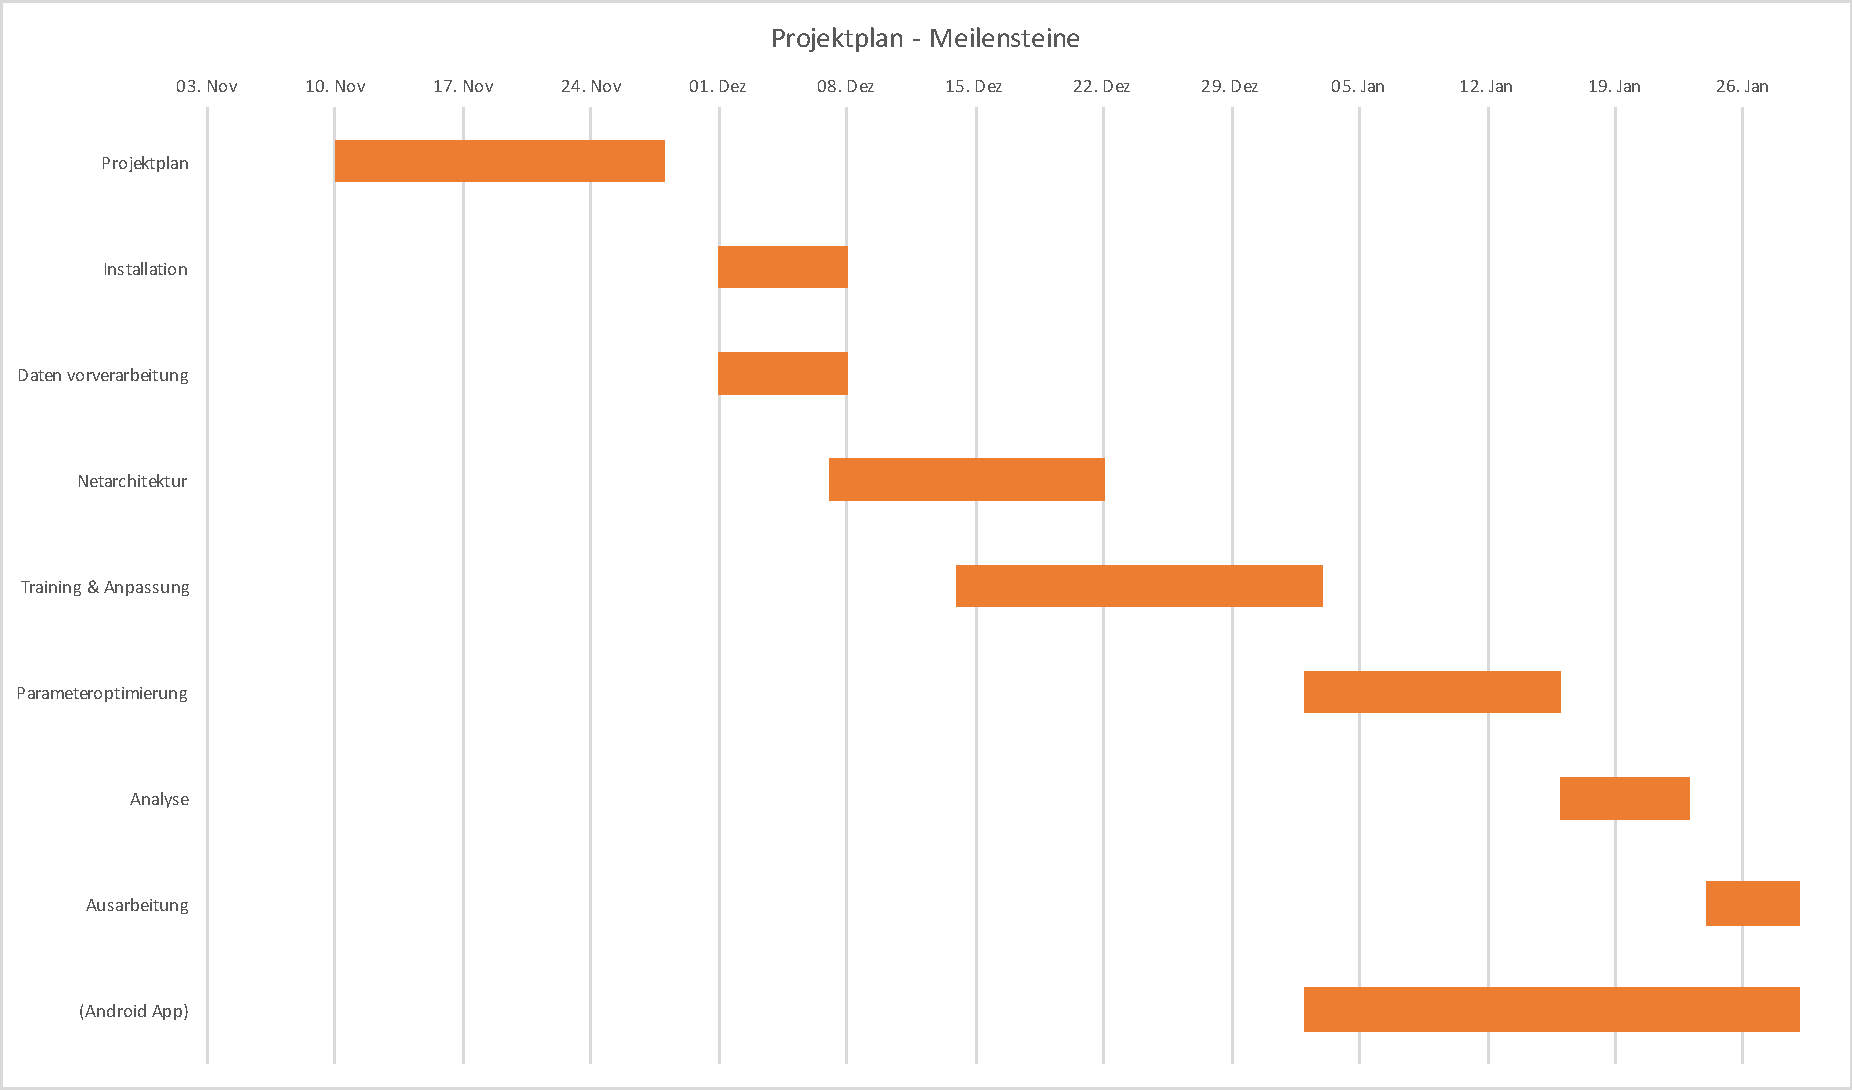
\includegraphics[width=\textwidth]{fig/gantt_projektplan}
 \caption{Meilensteine des Projekts als GANTT-Chart}
	\label{fig_gantt}
 \end{figure}

\section*{Tools}
Als Tools zur Umsetzung des Projekts, werden wir das Deep Learining Framework \textit{Tensorflow} \cite{tensorflow2015-whitepaper} in der Version 1.4 verwenden. Tensorflow bietet umfangreiche Möglichkeiten zur Implementierung und zum Training Neuronaler Netze. Zudem wird ein Deployment eines fertigen Netzes für eine Nutzung in einem Android System unterstützt.

Wir werden Python, die Python-API von Tensorflow 1.4 und möglicherweise die Python-Bibliotheken \textit{Pillow} und \textit{Numpy} für eine Vorverarbeitung der Daten nutzen.

Eine optionale Implementierung einer mobilen App, werden wir für Android in Java und den Bibliotheken aus Android Studio implementieren. 

\section*{Daten}

Die Autoren des Papers nutzen in ihrer Arbeit einen Datensatz von insgesamt 129.450 klinischen Bildern, die 2.032 verschiedene Krankheiten abbilden. All diese Krankheiten wurden in drei Unterklassen unterteilt: maligne, benigne und nicht-neoplastische, also nicht-tumoröse Krankheiten bzw. Läsionen. Aus diesem gesamten Datensatz wurden 127.463 Bilder für das Training und die Validierung genutzt und die restlichen 1.942 Bilder wurden zum Testen gebraucht. Die Daten stammten aus 18 verschiedenen Quellen, unter anderem aus dem ISIC Dermoscopic Archive \cite{ISIC}, welches ein freier Datensatz ist, der durch digitale Hautbilder dazu dienen soll die Sterblichkeitsrate bei Melanomen zu reduzieren. In unserer Ausarbeitung des Projekts werden wir unsere Daten ausschließlich aus diesem Datensatz beziehen, da sie frei erhältlich und für unsere Zwecke ausreichend sind. Somit verkleinert sich unsere Datenmenge auf 13.786 Bilder. Weiterhin werden wir zuerst lediglich eine Unterscheidung zwischen malignen und benignen Läsionen vornehmen und keine Einzelunterscheidungen zwischen den verschiedenen Krankheiten.\\
\noindent Die Bilder in dem ISIC Datensatz bestehen ausschließlich aus Aufnahmen von melanozytischen Hautläsionen, die anhand von Biopsien als maligne oder benigne Läsionen annotiert sind: 

\begin{figure}[h!]
	\centering
	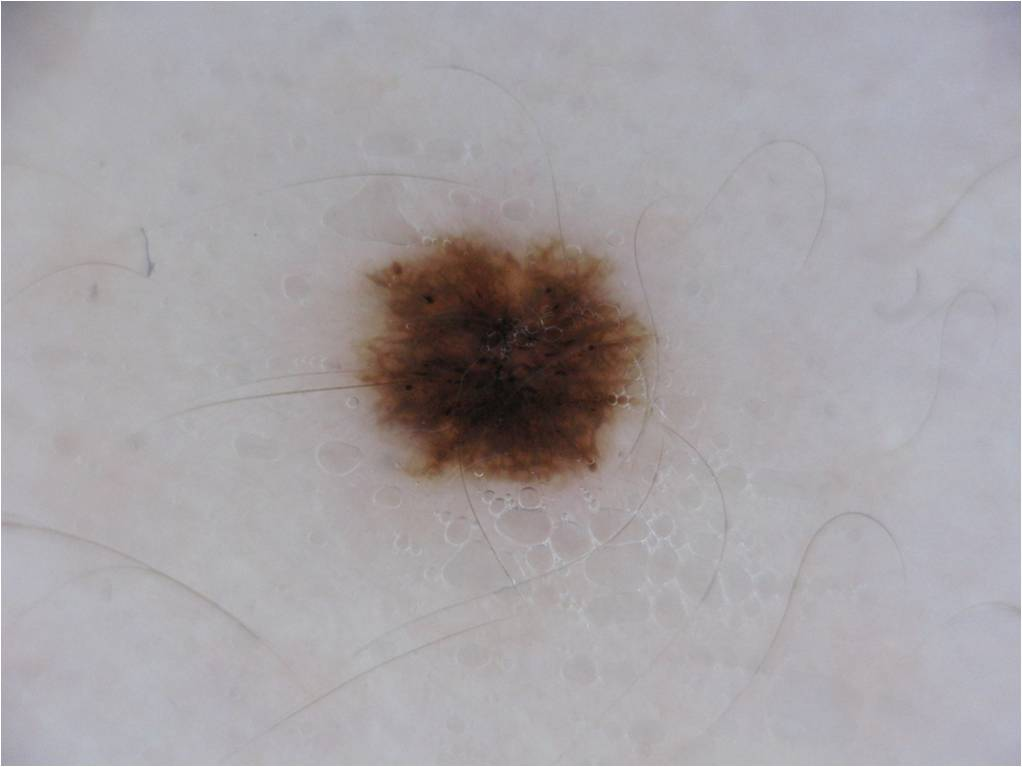
\includegraphics[width=0.2\textwidth]{fig/example1.jpg}
	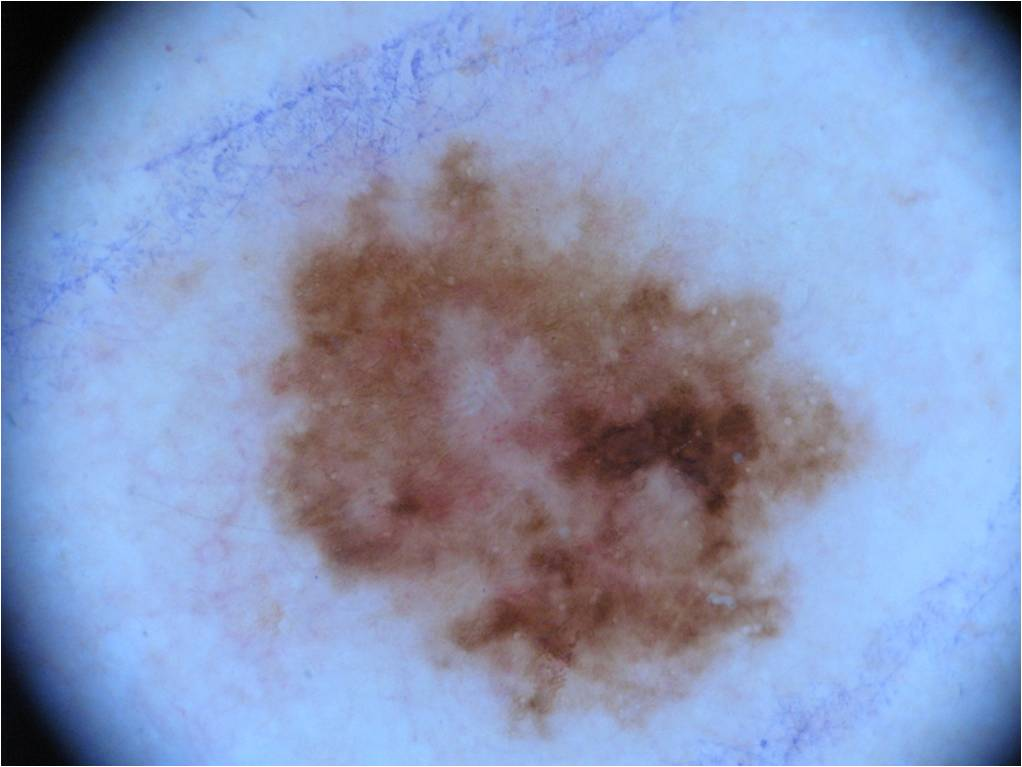
\includegraphics[width=0.2\textwidth]{fig/example2.jpg}
	\caption{Beispiele einer benignen (links) und einer malignen (rechts) Läsion.}
	\label{fig_example}
\end{figure}

\noindent Esteva et. al (2017) \cite{skincancer} sortierten bei ihrer Datenverarbeitung alle unscharfen Bilder und solche, die von zu weit weg aufgenommen aus. Zusätzlich beinhaltete ihr Datensatz auch Bilder der gleichen Läsion aus mehreren verschiedenen Blickwinkeln, was dem Training des Klassifizierers positiv beeinflusst hat. In unserem Fall tritt jede Läsion genau einmal auf, weswegen wir bei der Aufteilung des Datensatzes in Trainings- und Validierungsdaten, anders als die Autoren, auch keinen gesonderten Trenn-Algorithmus anwenden müssen, der dafür sorgt, dass zusammengehörige Bilder auch in das gleiche Subset kommen. Allerdings werden wir zur Verbesserung der Performanz unseres Klassifizierers alle Bilder sowohl in originaler Darstellung als auch in einer rotierten Darstellung präsentieren. Wir erhoffen uns dadurch einen stabileren Klassifizierer, der auch für die Anwendung in einer mobilen Android App geeignet wäre.\\
\noindent Zusammengefasst gestaltet sich unsere Datengewinnung und -verarbeitung etwas anders als die im originalen Paper von Esteva et. al (2017). Wir streben eine Vereinfachung des Klassifizierungsverfahrens an, indem wir nur zwischen zwei verschiedenen Klassen (maligne vs. benigne) unterscheiden und dafür insgesamt weniger Daten nutzen. Dies hat den Vorteil, dass wir anders als im Paper nicht auf die Mithilfe ausgebildeter Dermatologen angewiesen sind, die sich alle Bilder des Datensatzes einzeln ansehen müssten, um die Daten den 2.032 verschiedenen Krankheiten zuzordnen. Unser Ziel ist es einen generischen Klassifizierer zu finden, der dann für die jeweiligen Anwendungsfälle spezialisiert werden kann.   



\section*{Methode}

Analog zu \cite{skincancer} werden wir ein \textit{GoogleNet} in der \textit{Inception v3} \cite{inception} implementieren. Dazu werden wir ein fertiges Inception V3 Netz aus der \textit{tensorflow.contrib.slim} Bibliothek verwenden, welches für die ImageNet Large Scale Visual Recognition Challenge \cite{ILSVRC15} vor-trainiert wurde. Die vor-trainierten Gewichte werden von Slim zur Verfügung gestellt. 

\noindent Um das Neuronale Netz, welches für die ImageNet Challenge trainiert wurde, an unser Problem anzupassen, werden wir die letzten Layer des Inception V3 Netzes anpassen. Dazu entfernen wir die letzen Layer und ersetzen diese durch eine vollständig verbundene Schicht, mit einem Outputlayer von zwei Neuronen (maligne, benigne). 

\noindent Als Optimierer werden wir, analog zu Esteva et. al (2017) \cite{skincancer} anfangs RMSProp verwenden. Weitere Optimierer, wie beispielsweise Adam und SGD werden wir mit RMSProp vergleichen, um ein optimales Training zu gewährleisten.

\noindent Geplant ist, die Augmentierung der Daten in nativem Tensorflow Code zu implementieren und die Dataset-API von Tensorflow zu verwenden. Dies ermöglicht ein sehr effizientes Training. Jedoch werden wir als ersten Ansatz einen vereinfachte Methode zum Laden und Augmentieren der Daten umsetzen, um frühzeitig Netze trainieren zu können.

\noindent Als Fehlerfunktion während dem Training, werden wir anfangs einen einfachen 0,1-Loss nutzen. Es ist auch angedacht, andere Funktionen (L2-Loss) zu testen. 
 Zur Vermeidung von Overfitting werden wir, wie Estava et. al \cite{skincancer}, eine Kreuzvalidierung durchführen. 




\section*{Optional: Android App}
Damit der Klassifikator auch für jedermann nutzbar ist, soll falls wir noch genügend Zeit haben eine intuitiv bedienbare Android App entwickelt werden mit der ganz einfach über ein Foto gecheckt werden kann ob man zum Art gehen sollte oder der potentielle Hautkrebs harmlos ist.

\section*{Kontakt}
\centering
\begin{tabular}{lll}
\toprule
Name & Matrikelnummer & E-Mail Adresse \\
\midrule
Florence Lopez & 3878792  &  \href{mailto:florence.lopez@student.uni-tuebingen.de}{florence.lopez@student.uni-tuebingen.de} \\
Jonas Einig  & 3766150    & \href{mailto:jonas.einig@student.uni-tuebingen.de}{jonas.einig@student.uni-tuebingen.de}    \\
Julian Späth  & 3938726    & \href{mailto:julian.spaeth@student.uni-tuebingen.de}{julian.spaeth@student.uni-tuebingen.de}    \\
\bottomrule
\end{tabular}

\bibliography{mylit}
\bibliographystyle{unsrt}

\end{document}